\chapter{Introducción a GNU/Linux}
\section{Un poco de historia}
Para conocer cómo nació el movimiento GNU y el kernel Linux debemos conocer un poco de historia de la informática y cómo evolucionó en los primeros años.

\subsection{El nacimiento de Unix}

\begin{description}
\item[1964-1969]Los laboratorios \textbf{Bell} empiezan un proyecto con el \textbf{MIT} (Instituto Tecnológico de Massachusetts) y \textbf{General Electric} para desarrollar un sistema de \textbf{tiempo compartido} (“time-sharing computing”): se llamaría \textbf{Multics} (Multiplexed Information and Computing Service).

Hasta este momento, los sistemas utilizados eran de un único proceso, la CPU no era compartida por múltiples procesos sino que se ejecutaba por lotes (se les mandaba los procesos a ejecutar y se ejecutaban en orden).

Multics obtuvo licencia libre en el 2007. En Diciembre del 2016 salió la última versión 12.6f.

\itemimage{1969}{r}{0.33}
  {/Ken_Thompson_and_Dennis_Ritchie--1973.jpg}
  {\href{https://en.wikipedia.org/wiki/Ken_Thompson}{Ken y Dennis. Origen: Wikipedia}}
  {
  Uno de los desarrolladores de Multics, \href{https://en.wikipedia.org/wiki/Ken_Thompson}{Ken Thompson}, decidió escribir su propio sistema operativo. Ken Thompson es conocido también por crear el lenguaje de programación \textbf{B}, el sistema de codificación de caracteres UTF-8 y el lenguaje de programación Go, entre otras cosas.

A Ken Thompson se le une \href{https://en.wikipedia.org/wiki/Dennis_Ritchie}{Dennis Ritchie} y otros, y empiezan a programar un sistema de ficheros jerárquico, el concepto de procesos de computación, ficheros de dispositivos, un intérprete de comandos, … El resultado de lo programado era más pequeño y simple que Multics, lo que se convertiría en Unix. En Agosto ya tendrían el sistema operativo, se auto-gestiona,  tenía un assembler, un editor y una shell de comandos.

Dennis Ritchie es conocido también por crear junto con Ken el lenguaje de programación \textbf{C} (aparece por primera vez en 1972).
}


\item[1970]En ese momento el nuevo sistema operativo se llamaba \textbf{Unics} (\textit{Uniplexed Information and Computing Service}, un juego de palabras en contraposición a  Multics). No tenían todavía dinero de la organización en el desarrollo (era desarrollado por los programadores) y tampoco era multitarea todavía.

A finales de año el sistema ya era conocido como \textbf{UNIX}, y se había portado a la máquina PDP-11.

\textbf{Las primeras versiones de Unix incluían el código fuente} para que las universidades lo pudiesen modificar y así poder extenderlo a sus necesida des.


\item[1971]El sistema se empieza a hacer complejo y como querían que más usuarios lo usasen, crean el sistema de manuales que es utilizado hoy en día (mediante el comando \textbf{"man"}).

\begin{center}
  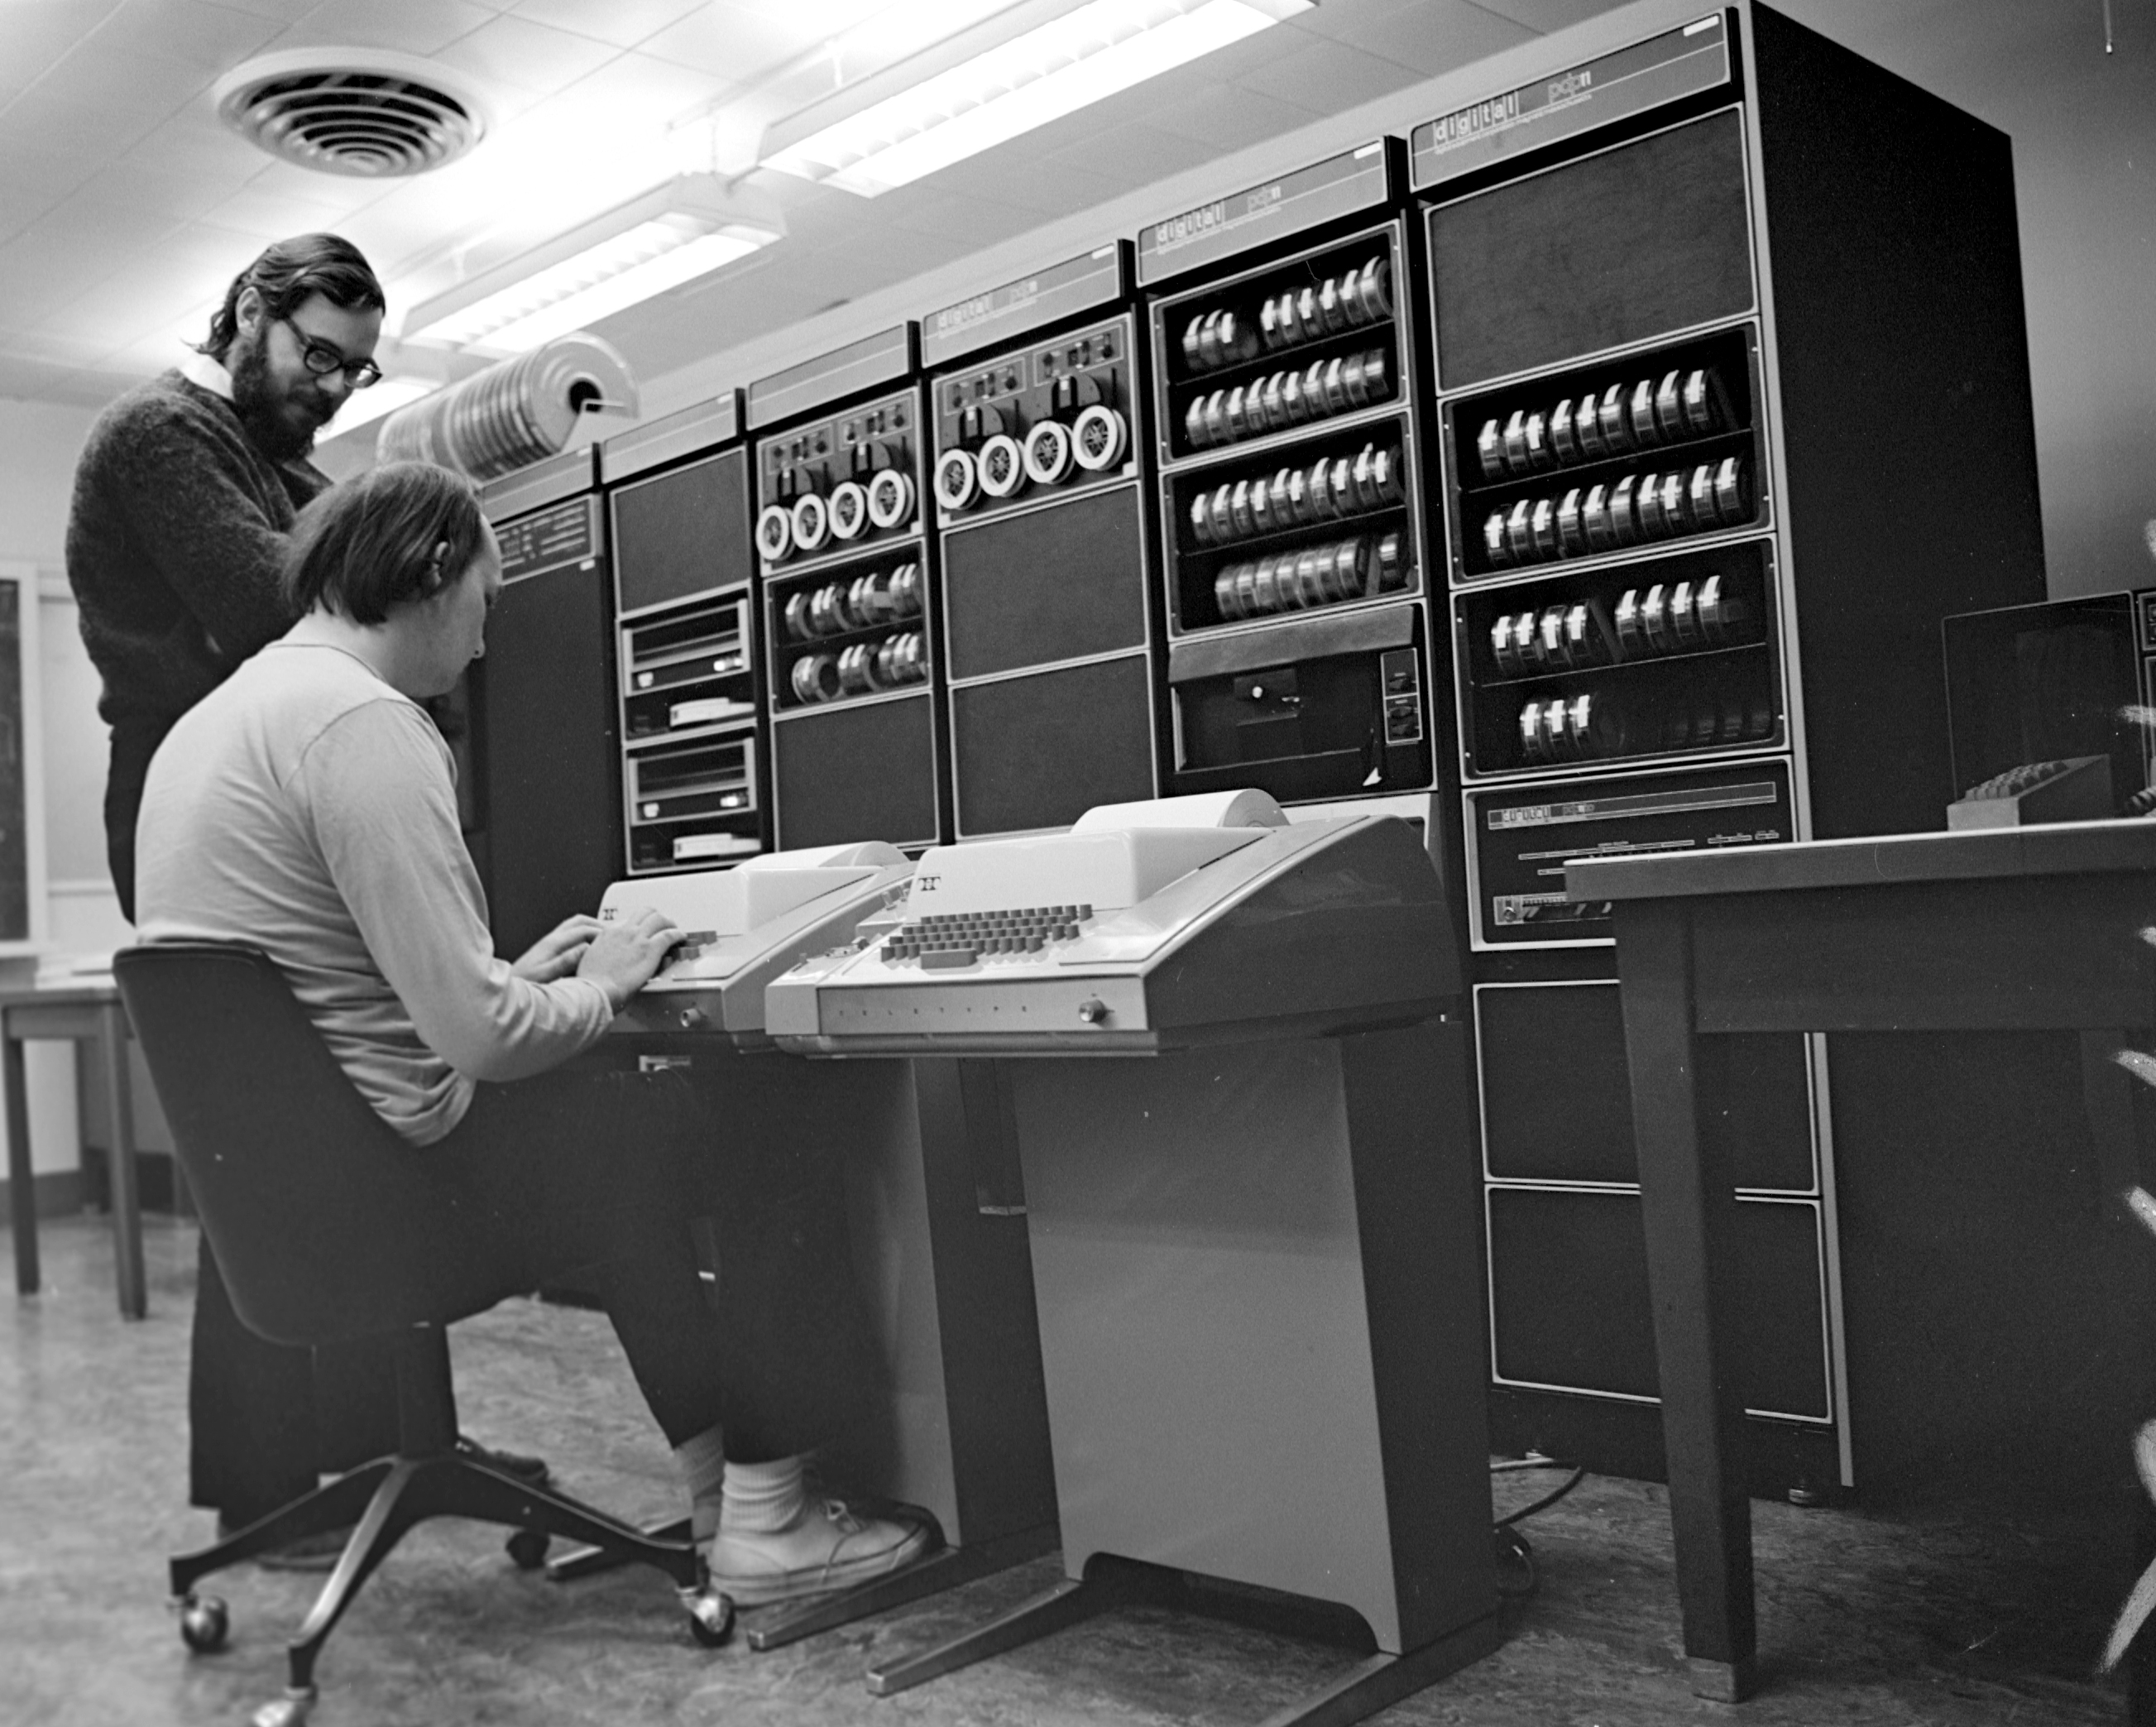
\includegraphics[width=0.8\linewidth]{/Ken_Thompson_(sitting)_and_Dennis_Ritchie_at_PDP-11_(2876612463).jpg}
  \vspace{-10pt}\captionof{figure}{\href{https://en.wikipedia.org/wiki/Ken_Thompson}{Dennis Ritchie y Ken Thompson trabajando en un PDP-11. Origen: Wikipedia}}\vspace{-13pt}
\end{center}


\item[1973]La versión 4 del sistema es reescrita completamente en C. Hasta este momento el sistema había estado escrito en ensamblador, por lo que no era portable entre distintos tipos de máquinas, aunque la primera versión portada a otra plataforma fue en 1978. Se cree que había “más de 20” instalaciones del sistema.

\item[1974]La versión 5 se licencia para ser utilizada en \textbf{instituciones educativas}.

\item[1975]La versión 6 se licencia para poder ser utilizadas por empresas por \$20.000 de la época.

\item[1977]La universidad de Berkeley lanza su primera versión de Unix bajo la Berkeley Software Distribution (BSD).

\item[1979]Con la salida de Unix v7, se comienza a portar a los distintos ``microordenadores'' de la época y a los distintos microprocesadores (Motorola 68000, Intel 8086, … ).

\item[1980]Microsoft anuncia su primer Unix para microcomputadoras de 16 bits (Xenix).
\end{description}

\subsection{El nacimiento de GNU (GNU's Not Unix}
\begin{description}

\item[1971]\href{https://en.wikipedia.org/wiki/Richard_Stallman}{Richard Stallman} comienza su carrera en el MIT en el laboratorio de inteligencia artificial.

Es conocido no sólo por el movimiento GNU, si no también por crear GCC y Emacs entre otra gran cantidad de software.

En esa época el software se distribuía de manera abierta para poder ser modificado. Lo habitual era realizar modificaciones para mejorar el software y distribuirlo entre compañeros y universidades.

\itemimage{1982}{r}{0.25}
  {/Richard_Stallman_2016_Talk_in_Madrid_06.jpg}
  {\href{https://commons.wikimedia.org/wiki/File:Richard_Stallman_2016_Talk_in_Madrid_06.jpg}{Richard Stallman: Wikimedia}}
  {
Richard Stallman quiere modificar el firmware de unas impresoras y el fabricante le pide que firme un acuerdo de no divulgación si le enseñan el código. Esto hace que Stallman se enfurezca y es cuando decide que la situación actual debe cambiar y volver al sistema de intercambio de software anterior.

\item[1983] Se anuncia el nacimiento del proyecto \textbf{GNU}, cuya finalidad es la de construir un sistema operativo completamente libre, compatible con Unix. La idea es dar a los usuarios la libertad y el control de sus ordenadores.

\item[1985] Se lanza el \href{https://www.gnu.org/gnu/manifesto.es.html}{manifiesto GNU}, y ya cuenta con un editor de texto (Emacs), compilador de C, una shell, varias utilidades … El núcleo inicial todavía no es funcional.
}


\item[1986]
Richard Stallman escribe y publica la definición de lo que es Free Software (Software Libre) a través de la \href{https://es.wikipedia.org/wiki/Free_Software_Foundation}{Free Software Foundation}.

\begin{tcolorbox}[title=Aclarando la palabra “free”:,sidebyside,righthand width=0.12\linewidth]

\textbf{The word “free” in our name does not refer to price; it refers to freedom.}

La palabra “free” no se refiere a gratis, si no que se refiere a libertad.

\tcblower

\includegraphics[width=\linewidth]{/gnu.png}
\end{tcolorbox}

Más adelante veremos a qué se refiere sobre libertad en el software.

\end{description}

\subsection{El nacimiento de Minix}
\begin{description}
\item[1987]Andrew S. Tanenbaum crea  Minix como propósito educativo y para enseñar cómo funciona un sistema operativo.

\item[1991]Sale la versión 1.5 de Minix y es portada a distintas arquitecturas (IBM, Motorola 68000, Amiga, Apple Macintosh, …).

\item[1992]Debate con Linus Torvalds sobre la arquitectura del kernel Linux (núcleo monolítico) en lugar de usar un micronúcleo.

\end{description}


\subsection{El nacimiento de Linux}
\begin{description}

\item[1991] Un estudiante en la universidad de Helsinki, \href{https://en.wikipedia.org/wiki/Linus_Torvalds}{Linus Torvalds}, comienza un proyecto personal escrito para su nuevo ordenador, un PC con procesador 80386.

El desarrollo comienza bajo \textbf{Minix}, usando el compilador \textbf{GCC} del movimiento GNU (GCC = GNU Compiler Collection).

El proyecto termina convirtiéndose en un kernel de un sistema operativo y escribió al grupo de noticias de Minix diciendo:

\begin{tcolorbox}[title=Email de Linus Torvalds presentando Linux,sidebyside,righthand width=0.30\linewidth]
  “Hola a todos los que estáis ahí fuera usando minix.\\


  Estoy haciendo un sistema operativo (libre), (solamente por aficion, no será grande ni profesional como el GNU) para clones 386(486) AT.

  ...

  PD. Sí – está libre de cualquier código de minix, y tiene un sistema de ficheros multi-hilo. NO es portable (usa el cambio de tareas del 386 etc), y probablemente nunca soporte otra cosa que no sean los discos duros AT, porque es todo lo que tengo :-(. ”
  \tcblower
  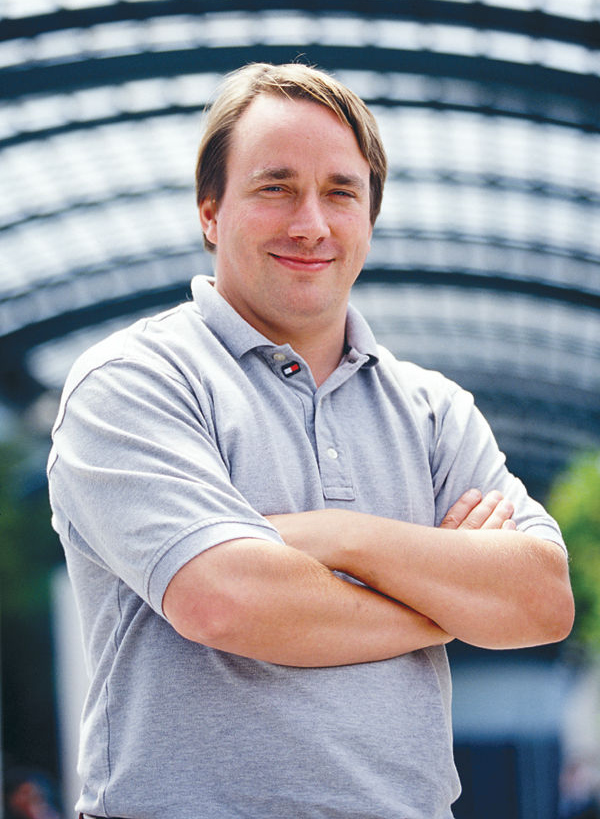
\includegraphics[width=\linewidth]{/Linus_Torvalds.jpeg}
  \vspace{-30pt}\captionof{figure}{\href{https://en.wikipedia.org/wiki/Linus_Torvalds}{Linus torvalds. Origen: Wikipedia}}
\end{tcolorbox}


\item[1992] Originalmente la licencia de Linux era propia e impedía el uso comercial de Linux. En la versión 0.99 esto cambia y se cambia a la licencia GNU Public License (\textbf{GPL}).

\item[1993] El proyecto cuenta con más de 100 desarrolladores. El kernel se adapta al entorno del proyecto GNU. Nace la distribución \textbf{Debian} (una de las más importantes a día de hoy)

\begin{center}
  
\includegraphics[width=0.5\linewidth]{/debian-logo.jpg}
  \vspace{-10pt}\captionof{figure}{\href{https://www.debian.org}{Debian}}
\end{center}

\item[1994] Se libera la versión 1.0. El proyecto XFree86 se une y Linux consigue interfaz gráfico. Nacen las primeras distribuciones comerciales \textbf{Red Hat} y \textbf{Suse}.

\item[1998] Empresas como \textbf{IBM}, \textbf{Compaq} y \textbf{Oracle} anuncian que apoyan a Linux. Nace el interfaz gráfico \textbf{KDE}.

\item[1999] Nace el interfaz gráfico \textbf{GNOME} como reemplazo a KDE, ya que KDE hacía uso de una librería propietaria en aquel momento (QT).

\item[2001] Steve Ballmer (CEO de Microsoft) dice: \textbf{“Linux es un cáncer”}.

\item[2002] Se libera OpenOffice (originalmente suite ofimática de Sun Microsystems). Nace Mozilla (hoy día:  Firefox).

\item[2003] IBM lanza un anuncio para la Linux Foundation: \href{https://www.youtube.com/watch?v=x7ozaFbqg00}{https://www.youtube.com/watch?v=x7ozaFbqg00}

\item[2004] Nace \textbf{Ubuntu} (basándose en Debian) y Steve Ballmer (CEO de Microsoft) dice que Linux infringe muchas de sus patentes.

\item[2008] Nace \textbf{\href{https://es.wikipedia.org/wiki/Android}{Android}}, sistema operativo con kernel Linux. Actualmente es el sistema operativo de móviles que más terminales tiene.

\item[2009] Red Hat iguala a Sun Microsystem en capitalización bursátil (un gran logro simbólico).

\item[2014] Satya Nadella (CEO de Microsoft) muestra en una presentación la siguiente transparencia:

\begin{center}
  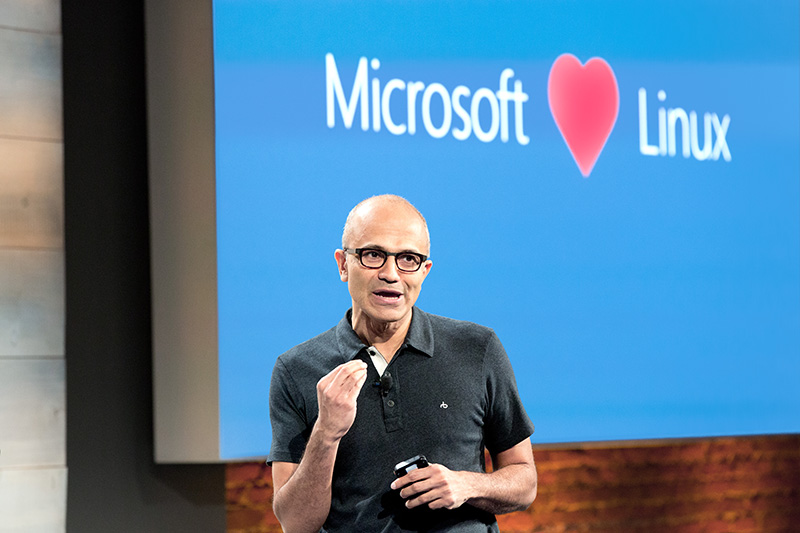
\includegraphics[width=0.5\linewidth]{/Microsoft_Linux.jpg}
  \vspace{-10pt}\captionof{figure}{\href{https://commons.wikimedia.org/wiki/File:Microsoft_Linux.jpg}{Origen: Wikipedia}}
\end{center}


\item[2016]
Microsoft anuncia \href{https://es.wikipedia.org/wiki/Windows_Subsystem_for_Linux}{WSL} (\textit{Windows Subsystem for Linux}) y se puede instalar en Windows 10 y Windows Server 2019. Permite correr ejecutables de Linux nativamente.

\end{description}

\subsection{Cronograma de sistemas Unix}
En el siguiente cronograma se puede ver la línea temporal de los sistemas Unix:

\begin{center}
  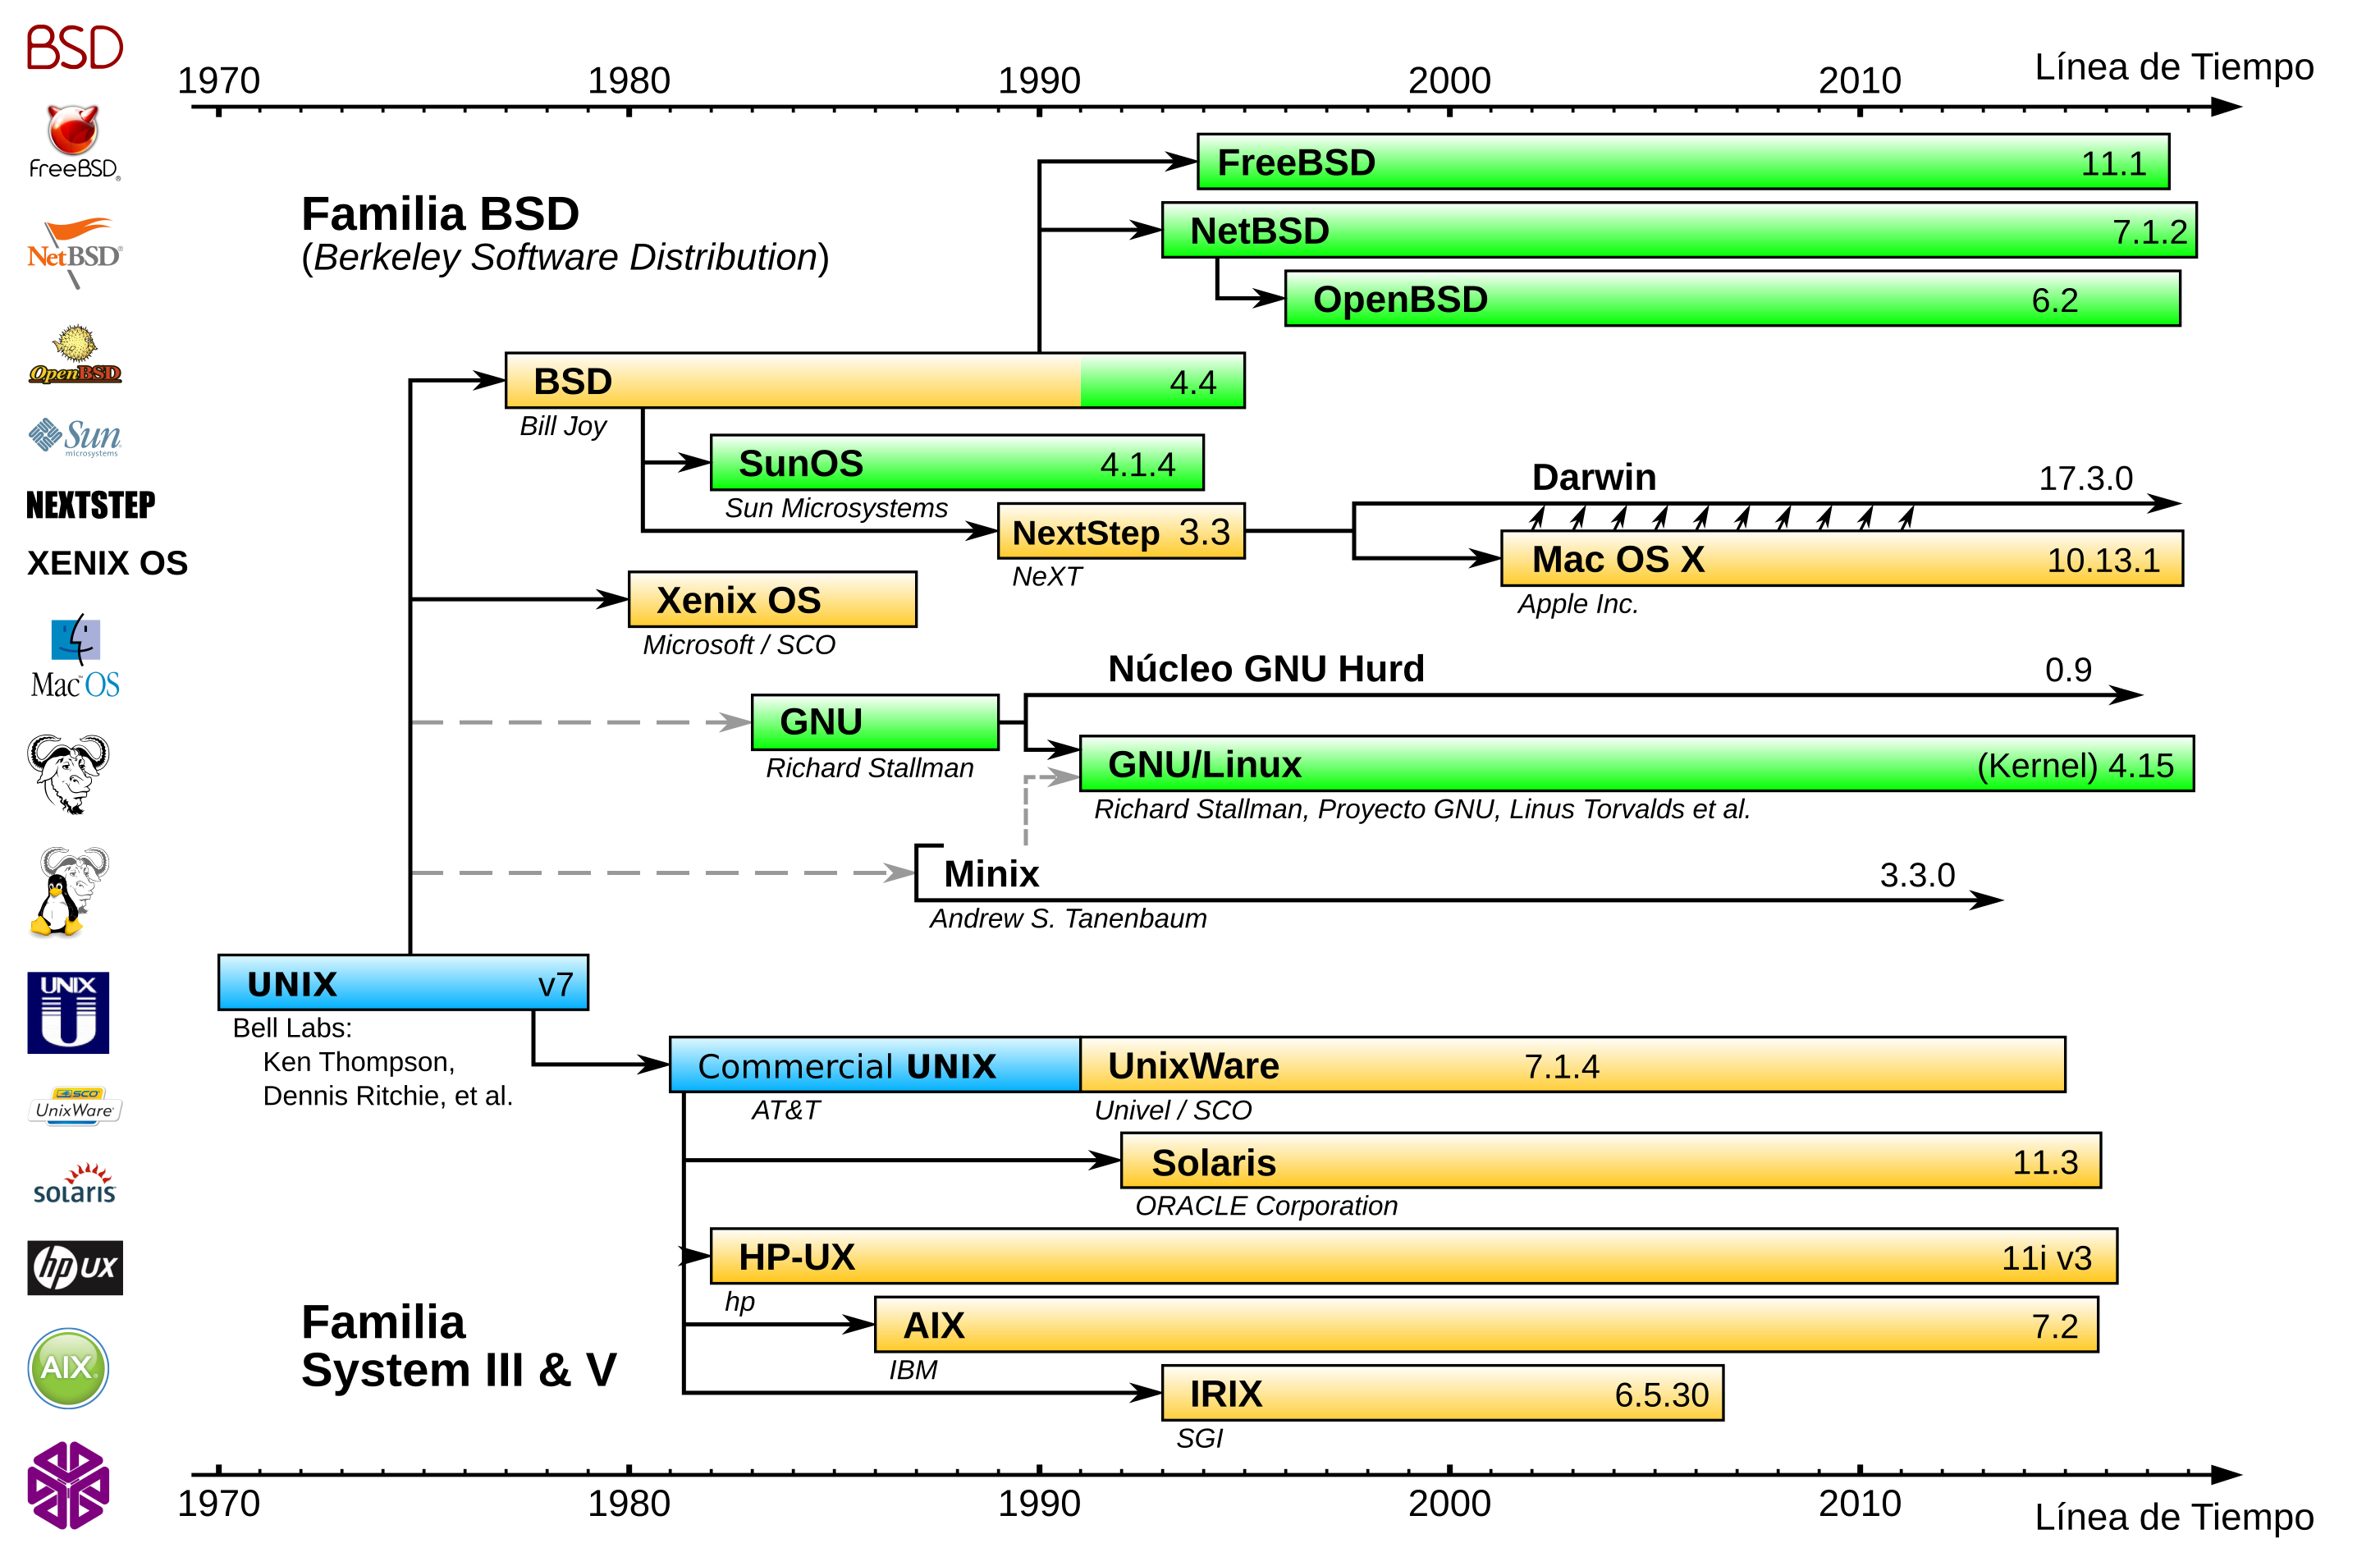
\includegraphics[width=0.7\linewidth]{/Evolución_UNIX.png}
  \vspace{-10pt}\captionof{figure}{\href{https://commons.wikimedia.org/wiki/File:Evolución_UNIX.png}{Origen: Wikipedia}}
\end{center}

\section{Resumen}
Linux es conocido como un sistema operativo libre pero el nombre de Linux se  centra única y exclusivamente en el \textbf{kernel} (o \textbf{núcleo}) del sistema operativo.

El sistema operativo completo debería llamarse \textbf{GNU/Linux}, ya que el kernel es una “pequeña” parte (aunque muy importante) dentro de todo el sistema operativo. El resto de herramientas utilizadas en el sistema operativo pertenecen al proyecto GNU.


\chapter{Licencias Libres}
%<*softwarelibre>
\section{Free Software / Software Libre}

En 1986 Richard Stallman saca a la luz la definición de lo que es Free Software (Software Libre) a través de la \href{https://es.wikipedia.org/wiki/Free_Software_Foundation}{Free Software Foundation}:

\begin{tcolorbox}[title=Aclarando la palabra “free”:,sidebyside,lower separated=false,righthand width=0.12\linewidth]

    \textbf{The word “free” in our name does not refer to price; it refers to freedom.} \linebreak

    La palabra “free” no se refiere a gratis, se refiere a \textbf{libertad}.

    \tcblower
    
\includegraphics[width=\linewidth]{/gnu.png}
\end{tcolorbox}


Las libertad en el software se refiere a:
\begin{tcolorbox}[title=Libertades del Software Libre:]
    \begin{enumerate}
        \setcounter{enumi}{-1}
        \item La libertad de ejecutar el programa, para cualquier propósito .

        \item La libertad de estudiar cómo trabaja el programa, y cambiarlo para que haga lo que usted quiera. El acceso al código fuente es una condición necesaria para ello.

        \item La libertad de redistribuir copias para que pueda ayudar al prójimo.

        \item La libertad de mejorar el programa y publicar sus mejoras, y versiones modificadas en general, para que se beneficie toda la comunidad. El acceso al código fuente es una condición necesaria.
    \end{enumerate}
\end{tcolorbox}

El movimiento del Free Software es un movimiento que tiene que ver más con la filosofía y la ética que con la tecnología en sí misma.


\subsection{Copyleft y GNU Public License (GPL)}
Es una práctica legal que consiste en el ejercicio del derecho de autor (copyright en inglés) con el objetivo de propiciar el libre uso y distribución de una obra, exigiendo que los concesionarios preserven las mismas libertades al distribuir sus copias y derivados (\href{https://es.wikipedia.org/wiki/Copyleft}{Wikipedia}).

\begin{center}
  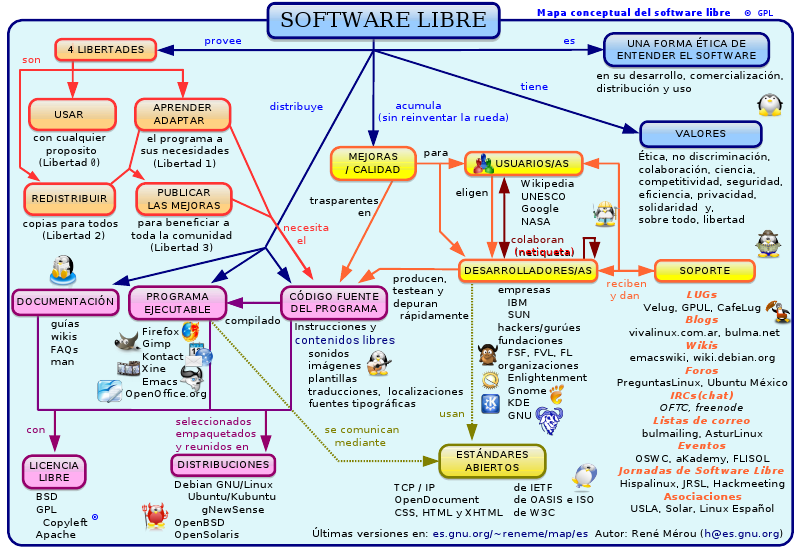
\includegraphics[width=\linewidth]{Mapa_conceptual_del_software_libre.png}
  \vspace{-30pt}\captionof{figure}{\href{https://commons.wikimedia.org/wiki/File:Mapa_conceptual_del_software_libre.png}{Mapa conceptual del Software Libre: Wikipedia}}\vspace{-20pt}
\end{center}

Con esto nació la licencia GNU GPL, la cual permite al usuario final la libertad de usar, estudiar, compartir y modificar el software recibido. Tiene que quedar claro que un programa comercial puede ser Software Libre.

\subsection{Diferencias con el Open Source}
Los programas Open Source son aquellos que podemos ver el código fuente pero esto no quiere decir que podamos modificarlo o adaptarlo a nuestras necesidades.

El Open Source es menos restrictivo que el Software Libre y se puede decir que todo Software Libre es Open Source, pero no todo Open Source tiene por qué ser libre.


\subsection{Licencias libres más conocidas}
Un listado de las licencias libres más utilizadas (en la \href{https://es.wikipedia.org/wiki/Anexo:Comparaci\%C3\%B3n_de_licencias_de_software_libre}{Wikipedia} existe una tabla comparativa):

\begin{itemize}
    \item \href{https://es.wikipedia.org/wiki/GNU_General_Public_License}{GNU GPL}
    \item \href{https://es.wikipedia.org/wiki/Licencia_BSD}{BSD}
    \item \href{https://es.wikipedia.org/wiki/Licencia_MIT}{MIT}
    \item \href{https://es.wikipedia.org/wiki/Apache_License}{Licencia Apache}
    \item \href{https://es.wikipedia.org/wiki/Licencia_PHP}{Licencia PHP}
    \item \href{https://es.wikipedia.org/wiki/Licencias_Creative_Commons}{Creative Commons} (no todas las versiones). Más utilizadas en contenido multimedia.
\end{itemize}
%</softwarelibre>

\chapter{Sistema de ficheros en GNU/Linux}
El sistema de ficheros en GNU/Linux, al igual que en Unix, es jerárquico, comenzando en la raíz denominada “/”. Partiendo de esta raíz, el resto del sistema de ficheros nace en forma de ramificaciones generando lo que se denominan “rutas de ficheros”, que es el camino completo para llegar al mismo.

\section{Filesystem Hierarchy Standard}
Debido a que en GNU/Linux todo se representa como ficheros (discos, dispositivos, programas, … ) es necesario que exista un orden a la hora de ser almacenados. Con esa intención nace en 1993 el estándar de la jerarquía de ficheros de Linux, enfocado a reestructurar los archivos. Posteriormente se unieron otros derivados de UNIX (la comunidad de desarrollo de BSD) por lo que terminó adoptando el nombre FHS.

Aún siendo un estándar, no todas las distribuciones lo siguen al pie de la letra, y otros Unix, como MacOS, tienen sus propias rutas especiales.


\section{Directorios importantes}
A continuación se exponen los directorios más importantes del sistema junto con la descripción del contenido que deben de tener:
\begin{itemize}

    \item \textbf{/boot/}: archivos de arranque del kernel, normalmente junto con la configuración utilizada para compilarlos.
    \item \textbf{/dev/}: contiene archivos especiales de bloque que representan los dispositivos del hardware que está corriendo el sistema operativo
    \item \textbf{/etc/}: contiene los archivos de configuración del servidor y de los servicios que corren en él. Está subdividido en directorios por servicios o configuraciones.
    \item \textbf{/home/}: los directorios de trabajo de los usuarios normales del sistema
    \item \textbf{/lib/}: librerías que hacen funcionar a los programas
    \item \textbf{/root/}: es la home del usuario root
    \item \textbf{/var/}: archivos variables del sistema
    \begin{itemize}
      \item \textbf{/var/lib/}: aquí se suelen guardar los ficheros de los programas que “crecen”: bases de datos, ficheros caché…
      \item \textbf{/var/log/}: los logs del sistema
    \end{itemize}
\end{itemize}

Junto a todos estos directorios, se ha separado los lugares en los que van los binarios, o ejecutables de los programas. Lo habitual es que se encuentren en estas rutas:

\begin{itemize}
    \item \textbf{/bin/}: aplicaciones esenciales del sistema
    \item \textbf{/sbin/}: aplicaciones que en principio sólo debería ejecutar el usuario root o programas de administración del sistema
    \item \textbf{/usr/bin/}: ejecutables de usuario
    \item \textbf{/usr/sbin/}: ejecutables de superusuario
\end{itemize}
Aunque las rutas de los ejecutables denotan quién debería ejecutar el programa, en la vida real no tiene por qué ser una limitación.

\section{Dispositivos de almacenamiento y discos duros}
En sistemas operativos Windows es habitual que cada partición cuente con una letra para acceder a ella, al igual que ocurre cuando introducimos un dispositivo de almacenamiento externo (un pendrive).

Tal como se ha comentado, en sistemas Unix el sistema de ficheros es una jerarquía, y por tanto todo dispositivo de almacenamiento nuevo deberá estar montado bajo la raíz “/”. Hoy día, en distribuciones con escritorio, al introducir un pendrive éste es auto-montado (es accesible) desde la ruta \textbf{/media/}, donde aparecerán tantos directorios como discos hayamos conectado.

\subsection{Almacenamiento permanente}
Si queremos que un disco duro nuevo sea permanente en nuestro sistema, podremos montarlo en cualquier lugar de la estructura jerárquica. Debido a este sistema, el usuario final no se tendrá que preocupar en almacenar los ficheros en una ruta distinta, si no que será el administrador el que haya hecho que esa ruta ahora pertenezca a un disco duro nuevo.

Imaginemos que el sistema operativo se ha instalado en un disco duro pequeño de 32Gb de espacio y se está llenando, y el directorio que más ocupa es el directorio de los usuarios. Podremos añadir al servidor un nuevo disco duro montado en /home y por tanto a partir de ahora los datos guardados en /home estarán en un nuevo disco duro más grande.

\begin{mycode}{Ejemplo de discos en un sistema con ``lsblk''`}{console}{}
root@vega:~# lsblk
NAME                       MAJ:MIN RM   SIZE RO TYPE MOUNTPOINTS
sda                          8:0    0   1,8T  0 disk
└─sda1                       8:1    0   1,8T  0 part /home/backup

sdb                          8:16   0   3,6T  0 disk
└─sdb1                       8:17   0   3,6T  0 part /home/disco4tb
sdc                          8:32   0 447,1G  0 disk
├─sdc1                       8:33   0   529M  0 part
├─sdc2                       8:34   0   100M  0 part
├─sdc3                       8:35   0    16M  0 part
└─sdc4                       8:36   0 446,5G  0 part
nvme0n1                    259:0    0 931,5G  0 disk
├─nvme0n1p1                259:1    0   512M  0 part
└─nvme0n1p2                259:2    0   800G  0 part /home
nvme1n1                    259:3    0 931,5G  0 disk
├─nvme1n1p1                259:4    0   512M  0 part /boot/efi
├─nvme1n1p2                259:5    0    90G  0 part /
├─nvme1n1p3                259:6    0   300G  0 part
│ ├─VMs-ubuntu--20.04--so1 254:0    0    10G  0 lvm
│ ├─VMs-manjaro            254:2    0    20G  0 lvm
│ └─VMs-win10              254:3    0    35G  0 lvm
└─nvme1n1p4                259:7    0 156,2G  0 part
\end{mycode}


\chapter{Gestión de usuarios locales en GNU/Linux}
En las distribuciones GNU/Linux lo habitual suele ser que existan al menos dos usuarios tras una instalación:

\begin{itemize}
    \item \textbf{root}: usuario administrador o súper usuario.
    \item \textbf{usuario no-privilegiado}: durante la instalación de la distribución nos suele preguntar para crear un usuario del sistema, que no tendrá privilegios.
\end{itemize}


El usuario root, como se ha dicho previamente, es el administrador del sistema, tiene permisos para realizar cualquier tarea dentro de nuestro sistema: instalar paquetes, desinstalarlos, modificar cualquier fichero, realizar formateos... Por lo tanto, el \textbf{realizar tareas como usuario root puede ser peligroso si cometemos algún fallo}.

Las buenas prácticas nos dicen que las tareas cotidianas del sistema deberíamos realizarlas como usuario normal y \textbf{sólo convertirnos en root cuando sea estrictamente necesario}.

\section{Creación de usuarios locales}

Tras instalar el sistema, veremos que se nos han creado varios usuarios en el sistema, aparte del usuario \textbf{root} y el usuario \textbf{no-privilegiado}. Para poder ver los usuarios que existen en nuestro sistema podemos verlo en el fichero \configfile{/etc/passwd} o podríamos obtener un listado ejecutando el siguiente comando:


\begin{mycode}{Listar usuarios del sistema}{console}{}
root@vega:~# cut -d: -f1 /etc/passwd
\end{mycode}

Para crear un usuario:

\begin{mycode}{Crear usuarios del sistema}{console}{\small}
root@vega:~# adduser ruben

Añadiendo el usuario `ruben' ...
Añadiendo el nuevo grupo `ruben' (1001) ...
Añadiendo el nuevo usuario `ruben' (1001) con grupo `ruben' ...
Creando el directorio personal `/home/ruben' ...
Copiando los ficheros desde `/etc/skel' ...
Nueva contraseña:
Vuelva a escribir la nueva contraseña:
passwd: contraseña actualizada correctamente
Cambiando la información de usuario para ruben
Introduzca el nuevo valor, o pulse INTRO para usar el valor predeterminado
    Nombre completo []:
    Número de habitación []:
    Teléfono del trabajo []:
    Teléfono de casa []:
    Otro []:
¿Es correcta la información? [S/n]
\end{mycode}

Y la línea que nos creará en el fichero  \configfile{ /etc/passwd }   es:
\begin{tcolorbox}[colback=white,title=Ejemplo de usaurio en “/etc/passwd”]
 \mintinline{console}{ ruben:x:1001:1001:ruben,,,:/home/ruben:/bin/bash }
\end{tcolorbox}

El fichero \configfile{ /etc/passwd }  nos muestra los datos de los usuarios, siendo un fichero que tiene distintos datos separados por “:”, siendo cada apartado:

\begin{center}
  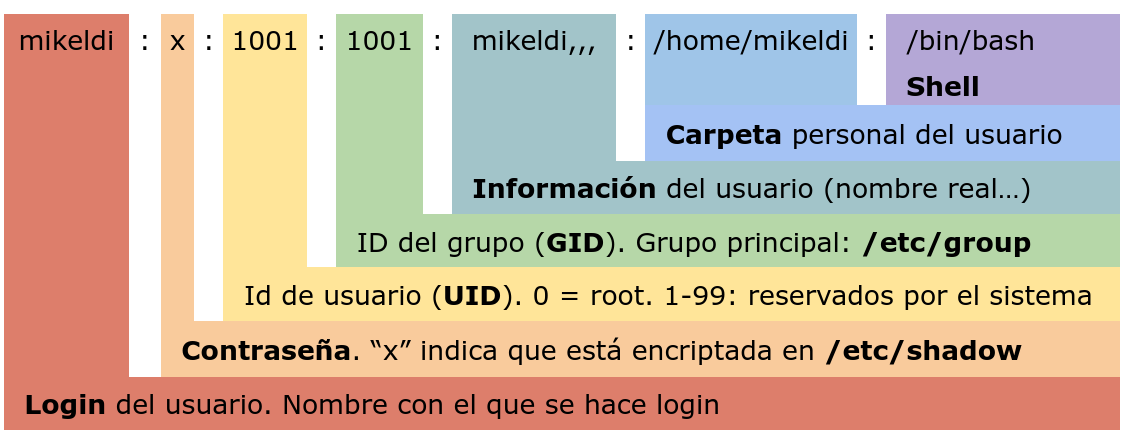
\includegraphics[width=0.7\linewidth]{usuario_tabla.png}
\end{center}


En las primeras versiones GNU/Linux la contraseña de los usuarios aparecía en el propio fichero /etc/passwd, lo que suponía un problema en la seguridad, ya que no estaban cifradas. Actualmente, las contraseñas de los usuarios se almacenan cifradas en el fichero \configfile{ /etc/shadow }. El fichero es similar al passwd, estando separados los apartados por “:”


\begin{center}
  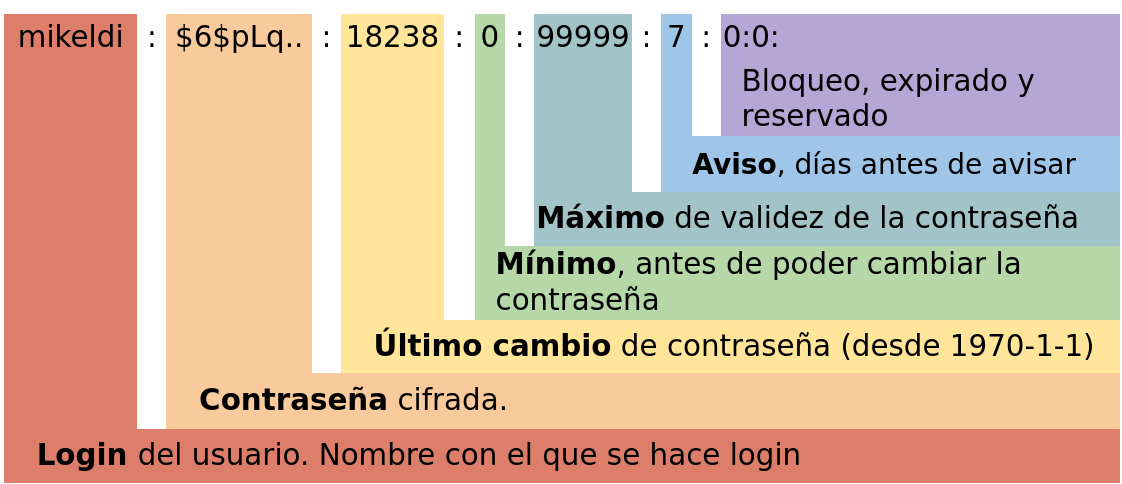
\includegraphics[width=0.7\linewidth]{shadow_tabla.png}
\end{center}


En el apartado de la contraseña podemos saber cierta información acerca de la misma ya que tiene el siguiente formato: \textbf{“\$id\$salt\$hashed”}
\begin{itemize}
    \item \textbf{id}: el algoritmo utilizado para cifrar la contraseña
    \begin{itemize}
        \item \$1\$ – MD5
        \item \$2a\$ – Blowfish
        \item \$2y\$ – Eksblowfish
        \item \$5\$ – SHA-256
        \item \$6\$ – SHA-512
    \end{itemize}
\end{itemize}

Aparte, también podemos encontrarnos con:
\begin{itemize}
    \item \textbf{Contraseña vacía}:  Si no hay contraseña, al pedirnos la contraseña a la hora de hacer login será suficiente con pulsar “intro”.
    \item \textbf{!}, \textbf{*}: la cuenta está bloqueada para la contraseña. El usuario no podrá loguearse utilizando la contraseña. Resulta útil si queremos bloquear el acceso con contraseña pero no con otros métodos (clave pública SSH).
    \item \textbf{*LK*}: cuenta bloqueda. El usuario no podrá loguearse.
    \item \textbf{*NP*}, \textbf{!!}: Nunca se ha puesto una contraseña
\end{itemize}


\section{Gestión de grupos}
En algunas distribuciones GNU/Linux, al crear un usuario directamente nos crea un grupo para el nuevo usuario. En otras, el usuario pertenece al grupo “users”.

Para saber los grupos a los que pertenece un usuario podemos ejecutar el comando \commandbox{ groups }. Los grupos del sistema aparecen en el fichero \configfile{ /etc/group }, y al igual que los ficheros vistos previamente, están separados por “\textbf{:}”.

\begin{center}
  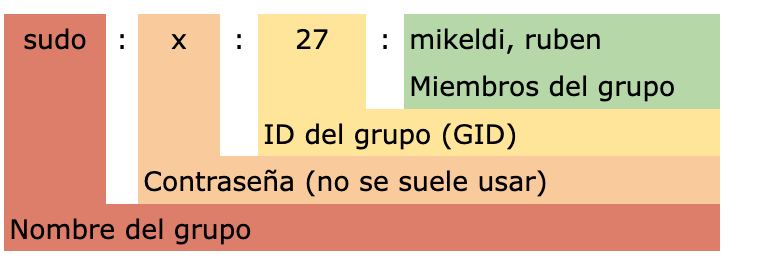
\includegraphics[width=0.6\linewidth]{grupo_tabla.png}
\end{center}

\section{Permisos de ficheros}
En GNU/Linux los ficheros cuentan con 3 tipos de permisos:
\begin{itemize}
    \item lectura (\textbf{r}ead): el usuario puede leer el fichero
    \item escritura (\textbf{w}rite): el usuario puede escribir en el fichero
    \item ejecución (e\textbf{x}ecute): el usuario puede el fichero o puede ver el contenido de un directorio
\end{itemize}


Todos ello para los distintos usuarios que pueden existir en el sistema:
\begin{itemize}
    \item \textbf{dueño del fichero}: la persona que ha creado el fichero
    \item \textbf{grupo}: los usuarios pertenecientes al grupo al que pertenece el fichero tendrán ciertos privilegios
    \item \textbf{el resto de usuarios}: los permisos que tendrán el resto de usuarios que no son ni el dueño ni pertenecen al grupo
\end{itemize}

Todo ello se puede visualizar en el sistema de ficheros si listamos los permisos del fichero:

\begin{mycode}{Ver los permisos de un fichero}{console}{}
ruben@vega:~$ ls -lh fichero.txt
-rw-r--r-- 1 ruben ruben 0 dic  8 19:17 fichero.txt
\end{mycode}

Los permisos se pueden ver en los primeros 10 caracteres:

\begin{center}
  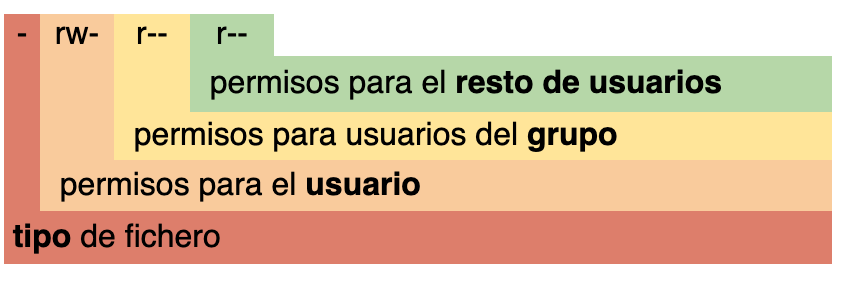
\includegraphics[width=0.7\linewidth]{permisos_fichero.png}
\end{center}

Existen los distintos tipos de ficheros:
\begin{itemize}
    \item \textbf{-} : fichero normal
    \item \textbf{d} : directorio
    \item \textbf{b} : dispositivo de bloque (ejemplo: /dev/sda*)
    \item \textbf{c} : dispositivo de carácter (las consolas. ejemplo: /dev/tty*)
    \item \textbf{s} : socket local
    \item \textbf{p} : tubería (pipe)
    \item \textbf{l} : enlace simbólico (link)
\end{itemize}

\subsection{Permisos especiales}

Existen otros permisos especiales:
\begin{itemize}
    \item \textbf{SUID}: permiso especial que permite que el fichero sea ejecutado con los permisos del dueño del fichero (aunque lo ejecute otro usuario). Se visualiza con una “S” en el permiso de ejecución del dueño  \texttt{-rwSrw-r- -} .
%% TODO: modificar los fondos de los permisos
    \item \textbf{SGID}: permiso especial que permite que el fichero sea ejecutado como el grupo. Aparece una “S” en el permiso de ejecución del grupo: \texttt{-rwx- -S- - -}.

    \item \textbf{STICKY}: si el bit sticky está activado en un directorio sólo el usuario root, el dueño del directorio o el dueño del fichero puede borrar ficheros de dicho directorio. Aparece una “t” en el permiso de ejecución del resto de usuarios: \inlineconsole{d-rwx-rx-r-t}.

\end{itemize}

\subsection{Cambiando permisos y dueños a los ficheros y a los directorios}

Para cambiar los permisos a los ficheros y a los directorios se hace con el comando \textbf{chmod}.

Para cambiar permisos de dueño a los ficheros y a los directorios se hace con el comando \textbf{chown}.

\section{La importancia de “sudo”}
En muchas distribuciones GNU/Linux el usuario no-privilegiado que se crea tiene permiso de “sudo” para poder ejecutar comandos como si se tratara del \textbf{root} (u otro usuario) para poder realizar tareas de administración. Es habitual que en estas distribuciones \textbf{el usuario root no suela tener contraseña}.

Cuando un usuario necesite realizar una tarea como administrador, deberá usar “sudo” antes del comando:

\begin{mycode}{Editar un fichero con permisos de root}{console}{}
ruben@vega:~$ sudo nano /etc/passwd
\end{mycode}

Tras realizar este comando, el sistema nos pedirá la contraseña del usuario con el que lo estemos ejecutando y comprobará que el usuario tiene permisos de “sudo” para poder ejecutar el comando (en este caso: nano).

El comando “\textbf{sudo}” viene de “\textbf{su}per user \textbf{do}” (que en inglés sería: “super usuario haz”), y aunque su uso habitual es el de permitir realizar cualquier comando de administración, la configuración permite mucho más, pudiendo permitir a ciertos usuarios sólo realizar ciertas tareas. Por ejemplo:

\begin{itemize}
    \item Usuario \textbf{ruben}: tendría permisos para poder realizar cualquier comando del sistema.
    \item Usuario \textbf{dba}: sólo tendría permisos para poder realizar el reinicio del sistema de base de datos.
    \item Usuario \textbf{adminweb}: sólo tendría permisos para poder realizar el reinicio del servidor web.
    \item ....
\end{itemize}

De esta manera, la gestión de nuestro servidor estaría basada en múltiples usuarios y cada usuario sólo sería capaz de realizar pequeñas tareas, por lo que la seguridad del servidor sería mayor y limitaría lo que los usuarios puedan realizar.

\subsection{Configurando “sudoers”}
Los permisos de sudo se realizan en el fichero  \configfile{/etc/sudoers} , y para su edición se hace uso del comando \textbf{visudo}, el cual abre el fichero y se asegura que a la hora de guardar la sintaxis es correcta.

Si realizamos cualquier modificación sobre el fichero, éste será tenido en cuenta la próxima vez que se realice la ejecución del comando “sudo”, por lo tanto, no hay que realizar ningún reinicio de servicio.

El fichero \configfile{/etc/sudoers}  tiene permisos de sólo lectura para el usuario root y el grupo root:

\begin{mycode}{Permisos del fichero \faFile \hspace{1pt} /etc/sudoers}{console}{}
root@vega:# ls -lh /etc/sudoers
-r--r----- 1 root root 669 jun  5  2017 /etc/sudoers
\end{mycode}

Un fichero sudoers suele tener el siguiente aspecto:

\begin{mycode}{Contenido del fichero \faFile \hspace{1pt} /etc/sudoers}{bash}{\footnotesize}
Defaults    env_reset
Defaults    mail_badpass
Defaults    secure_path="/usr/local/sbin:/usr/local/bin:/usr/sbin:/usr/bin:/sbin:/bin"

# User privilege specification
root    ALL=(ALL:ALL) ALL

# Allow members of group sudo to execute any command
%sudo   ALL=(ALL:ALL) ALL

# See sudoers(5) for more information on "#include" directives:

#includedir /etc/sudoers.d
\end{mycode}

La línea que más importa en este fichero es la que indica “\textbf{\%sudo   ALL=(ALL:ALL) ALL}” y es explicada en su comentario anterior. Lo que quiere decir es que cualquier usuario que pertenezca al grupo “sudo” podrá realizar cualquier comando del sistema como superusuario. La sintaxis de la línea es:

\begin{itemize}
    \item \textbf{\%sudo}:  cualquier usuario que pertenezca al grupo “sudo”
    \item \textbf{ALL}= : desde cualquier host o IP
    \item \textbf{(ALL:ALL)}: el usuario que ejecuta puede ejecutar el comando como cualquier usuario y cualquier grupo
    \item \textbf{ALL}: puede ejecutar cualquier comando
\end{itemize}

Un ejemplo limitando el uso de sudo a un único comando a un usuario:

\begin{mycode}{Añadimos configuración al fichero \faFile \hspace{1pt} /etc/sudoers}{bash}{}
ruben    ALL=(ALL:ALL) NOPASSWD:/bin/systemctl suspend
\end{mycode}

Con esta línea lo que estamos permitiendo es que el usuario “ruben” puede ejecutar el comando “/bin/systemctl suspend” (suspender el equipo) y sin necesidad de meter contraseña al hacer sudo, gracias a la opción “NOPASSWD”).

\section{Diferencias entre “sudo”, “su” y “su -”}
Como ya se ha comentado en el apartado anterior, “sudo” permite la ejecución de comandos como cualquier usuario, siendo lo habitual ejecutarlo como root. Ahora bien, en entornos donde el usuario root tiene contraseña, nos puede interesar convertirnos en él para realizar tareas sin tener que estar ejecutando “sudo” a cada comando. Al ser root, tendremos que tener especial cuidado.

\subsection{Variables de entorno}
En cualquier sistema operativo existen las denominadas “variables de entorno”. Son variables que cada usuario tiene y sirven para indicar ciertos parámetros que se están utilizando (la SHELL que se está usando), o parámetros que se van a usar a la hora de ejecutar comandos o realizar tareas, ya que se consultan a ellas. En GNU/Linux las variables de entorno se pueden consultar ejecutando:

\begin{mycode}{Vemos las variables de entorno del usuario ruben}{console}{}
ruben@vega:~$ printenv
LANG=es_ES.utf8
LOGNAME=ruben
XDG_VTNR=2
COLORTERM=truecolor
PWD=/home/ruben
DESKTOP_SESSION=gnome
USERNAME=ruben
SHELL=/usr/bin/zsh
PATH=/usr/local/bin:/usr/bin:/bin:/usr/local/games:/usr/games
...
\end{mycode}

Una variable de entorno puede consultarse haciendo:

\begin{mycode}{Consultamos el contenido de la variable \$PATH}{bash}{}
ruben@vega:~$ echo $PATH
/usr/local/bin:/usr/bin:/bin:/usr/local/games:/usr/games

\end{mycode}

Como se puede ver, es con un “\textbf{\$}” y el nombre de la variable en mayúsculas. Existen muchas variables de entorno, y podríamos crear las nuestras propias si así lo necesitáramos.

\subsection{La importancia de “su -”}
Con el comando “\textbf{su}” nos podemos convertir en cualquier otro usuario del sistema siempre y cuando \textbf{conozcamos su contraseña}. Hay que notar la diferencia respecto a “\textbf{sudo}” que cuando lo ejecutamos nos pide \textbf{nuestra contraseña}.

\textbf{Al ejecutar “su” nos convertimos en el usuario root} (o ejecutando “su usuario2”, nos convertimos en el usuario2), \textbf{pero no hacemos uso de sus variables de entorno}, si no que seguimos  con las variables de entorno del usuario que éramos previamente.
Para convertirnos en el usuario y que obtengamos sus variables de entorno es necesario ejecutar “\textbf{su -}”, o lo que es lo mismo: “\textbf{su -l}”, que el manual nos dice: “\textit{Start the shell as a login shell with an environment similar to a real login}”. Por ejemplo:

\begin{mycode}{Consultamos el contenido de la variable \$PATH en distintas situaciones}{bash}{}
ruben@vega:~$ echo $PATH
/usr/local/bin:/usr/bin:/bin:/usr/local/games:/usr/games

ruben@vega:~$ su
Contraseña:

root@vega:/home/ruben# echo $PATH
/usr/local/bin:/usr/bin:/bin:/usr/local/games:/usr/games

root@vega:/home/ruben# exit

ruben@vega:~$ su -
Contraseña:

root@vega:~# echo $PATH
/usr/local/sbin:/usr/local/bin:/usr/sbin:/usr/bin:/sbin:/bin

\end{mycode}

El usuario “ruben” tiene unos valores en la variable de entorno PATH (es la variable que se encarga de tener las rutas de los ejecutables de los programas). Al convertirse en root haciendo uso de “su”, y mirar la variable PATH, podemos observar que es igual que el usuario prueba.

Ahora bien, si a la hora de convertirse en root hace uso de “su -”, se puede ver cómo la variable PATH obtiene otros valores, siendo lo más significativo que aparecen las rutas “/usr/local/sbin” y “/usr/sbin” que son las rutas donde se almacenan los ejecutables que (en principio) sólo deberían ejecutarse como administrador del sistema.


